\documentclass[preprint,12pt]{elsarticle}

\usepackage{booktabs}
\usepackage{amsmath,amssymb}
\usepackage{graphicx}
\usepackage{multirow}
\usepackage{siunitx}
\usepackage{hyperref}
\usepackage{enumitem}
\usepackage{float}

\journal{Neurocomputing}

\begin{document}

\begin{frontmatter}

\title{Physics-Guided Satellite Data Assimilation with Spectral Adaptation and Gated Fusion: A Reproducible Ablation-Centric Study}

\author{First Author}
\author{Second Author}
\address{School of XXX, University of XXX, City, Country}

\begin{abstract}
Satellite radiance assimilation requires jointly handling multi-source heterogeneity, sparse/irregular observations, and vertically coupled atmospheric structure. We present a physics-guided deep assimilation framework implemented in a distributed training pipeline and validated by systematic ablation. The model ingests satellite observations, ERA5 background, and optional auxiliary geophysical features, then predicts analysis increments on 37 pressure levels. The core design combines a spectral-adapter stem, mask-aware processing, and gated fusion before a U-Net style encoder-decoder. On the 64x64 test set (387 samples), our best variant (V1, no auxiliary branch) achieves \textbf{1.1696 K RMSE}, improving over ERA5 background (1.8230 K) by \textbf{35.84\%}. Full variant reaches 1.2674 K (+30.48\%), while standard comparison baselines (VanillaUNet, FuXi-DA, AttentionUNet, PixelMLP, ResUNet) remain clearly behind. We provide a paper-ready draft with reproducible settings, complete ablation discussion, and figure integration from the code-generated assets.
\end{abstract}

\begin{keyword}
Satellite data assimilation \sep Physics-guided deep learning \sep Ablation study \sep U-Net \sep Distributed training
\end{keyword}

\end{frontmatter}

\section{Introduction}
Data assimilation is central to numerical weather prediction, but operational pipelines often face two practical bottlenecks: (i) nonlinear mapping between radiance observations and atmospheric states, and (ii) robustness degradation under missing or sparse observations. Recent deep assimilation approaches alleviate computational cost, yet may underperform without strong inductive biases.

This work targets a practical, code-grounded pipeline that is reproducible and publication-ready. The framework is implemented with PyTorch DistributedDataParallel (DDP), mixed precision, and configurable model variants for strict ablation. Unlike purely empirical comparisons, our focus is to map architectural decisions to measurable impact.

Our main contributions are:
\begin{enumerate}[leftmargin=*]
\item A physics-guided assimilation architecture coupling spectral adaptation, mask-aware modeling, and gated fusion in a unified stem + U-Net backbone.
\item A reproducible DDP training/evaluation framework supporting increment learning, multiple loss types, and controlled ablations.
\item A broad comparison suite (B2--B7) and ablations (V1--V4), including newly added AttentionUNet, PixelMLP, and ResUNet baselines.
\item A clear empirical finding for this 64x64 setup: the V1 variant (without auxiliary branch) is the best-performing configuration and should be treated as the primary model in this domain scale.
\end{enumerate}

\section{Method}
\subsection{Problem formulation}
For each sample, inputs are observation $\mathbf{x}_{obs}\in\mathbb{R}^{17\times H\times W}$, background field $\mathbf{x}_{bkg}\in\mathbb{R}^{37\times H\times W}$, validity mask $\mathbf{m}\in\mathbb{R}^{1\times H\times W}$, and optional auxiliary fields $\mathbf{x}_{aux}\in\mathbb{R}^{4\times H\times W}$. The model predicts normalized increment $\hat{\Delta}\in\mathbb{R}^{37\times H\times W}$.

Analysis in physical units is reconstructed as:
\begin{equation}
\hat{\mathbf{a}} = \mathbf{x}_{bkg}^{phys} + \mathrm{InvNorm}_{inc}(\hat{\Delta}).
\end{equation}

\subsection{Physics-guided backbone}
The primary model is \texttt{PhysicsAwareUNet} with:
\begin{enumerate}[leftmargin=*]
\item \textbf{SpectralAdapterStemV2}: projects observations/background to latent channels and fuses them using one of \{concat, add, gated\}.
\item \textbf{Mask-aware processing}: observation features are explicitly modulated by validity mask to mitigate missing-data artifacts.
\item \textbf{Encoder-decoder}: channels \{64,128,256,512\} in encoder and \{256,128,64,64\} in decoder.
\item \textbf{Attention bottleneck}: optional CBAM in bottleneck to enhance channel/spatial selectivity.
\item \textbf{Residual output path}: direct background skip improves optimization stability.
\end{enumerate}

\subsection{Training objective}
The framework supports \texttt{mse}, \texttt{mae}, \texttt{huber}, and \texttt{combined} losses. For combined loss:
\begin{equation}
\mathcal{L}=\mathcal{L}_{base}+\lambda_g\mathcal{L}_{grad}+\lambda_d\mathcal{L}_{deep},
\end{equation}
where $\mathcal{L}_{grad}$ is computed using Sobel gradients and $\mathcal{L}_{deep}$ is optional deep supervision.

\subsection{Compared models}
\textbf{Ablations}: Full, V1 (w/o Aux), V2 (w/o MaskConv), V3 (w/o GatedFusion), V4 (w/o SpectralStem).\\
\textbf{Comparisons}: B2 (OI/1DVar), B3 (VanillaUNet), B4 (FuXi-DA), B5 (AttentionUNet), B6 (PixelMLP), B7 (ResUNet).

\section{Experimental setup}
\subsection{Data and protocol}
Experiments use 64x64 samples with 17 observation channels and 37 pressure levels. Test split includes 387 files. We report RMSE, MAE, Bias, Correlation, and improvement over ERA5 background.

\subsection{Implementation details}
Training uses DDP with \texttt{torchrun}, optional \texttt{SyncBatchNorm}, AMP (\texttt{GradScaler}), AdamW, and cosine/one-cycle scheduler options. Increment learning is enabled via precomputed increment statistics.

Default practical setting for main runs:
\begin{itemize}[leftmargin=*]
\item Epochs: 200
\item Batch size: 16 per GPU
\item Optimizer: AdamW
\item Scheduler: cosine
\item Objective: increment prediction
\end{itemize}

\section{Results}
\subsection{Overall comparison}
Table~\ref{tab:main} summarizes results from the generated evaluation CSV.

\begin{table}[H]
\centering
\caption{Main quantitative results on the 64x64 test set. Lower RMSE/MAE is better.}
\label{tab:main}
\begin{tabular}{lccccc}
\toprule
Method & Type & RMSE (K) & MAE (K) & Corr & Improve (\%) \\
\midrule
Background (ERA5) & bkg & 1.8230 & 1.8230 & 0.00000 & +0.00 \\
OI/1DVar (B2) & oi & 1.8836 & 1.2798 & 0.00000 & -3.32 \\
Full & full & 1.2674 & 0.8650 & 0.99832 & +30.48 \\
\textbf{V1 (w/o Aux)} & ablation & \textbf{1.1696} & \textbf{0.8054} & \textbf{0.99858} & \textbf{+35.84} \\
V2 (w/o MaskConv) & ablation & 1.2150 & 0.8337 & 0.99849 & +33.35 \\
V3 (w/o GatedFusion) & ablation & 1.3734 & 0.9445 & 0.99736 & +24.66 \\
V4 (w/o SpectralStem) & ablation & 1.4265 & 0.9690 & 0.99732 & +21.75 \\
VanillaUNet (B3) & compare & 1.4491 & 1.0093 & 0.99684 & +20.51 \\
FuXi-DA (B4) & compare & 1.4095 & 0.9995 & 0.99654 & +22.68 \\
AttentionUNet (B5) & compare & 1.5092 & 1.0508 & 0.99666 & +17.21 \\
PixelMLP (B6) & compare & 1.6498 & 1.1277 & 0.99658 & +9.50 \\
ResUNet (B7) & compare & 1.5407 & 1.0784 & 0.99630 & +15.49 \\
\bottomrule
\end{tabular}
\end{table}

\subsection{Ablation insights}
The ranking supports three key observations:
\begin{enumerate}[leftmargin=*]
\item \textbf{V1 outperforms Full}: auxiliary branch is not beneficial in this small-domain setup.
\item \textbf{Spectral stem matters}: removing it (V4) causes large degradation.
\item \textbf{Gated fusion is effective}: replacing gated fusion with simple addition (V3) significantly increases error.
\end{enumerate}

\begin{figure}[H]
\centering

\includegraphics[width=0.9\linewidth]{../prediction/paper_figures/fig_combined_rmse_improve.png}
\caption{Combined RMSE and improvement comparison across all methods.}
\label{fig:combined}
\end{figure}

\begin{figure}[H]
\centering
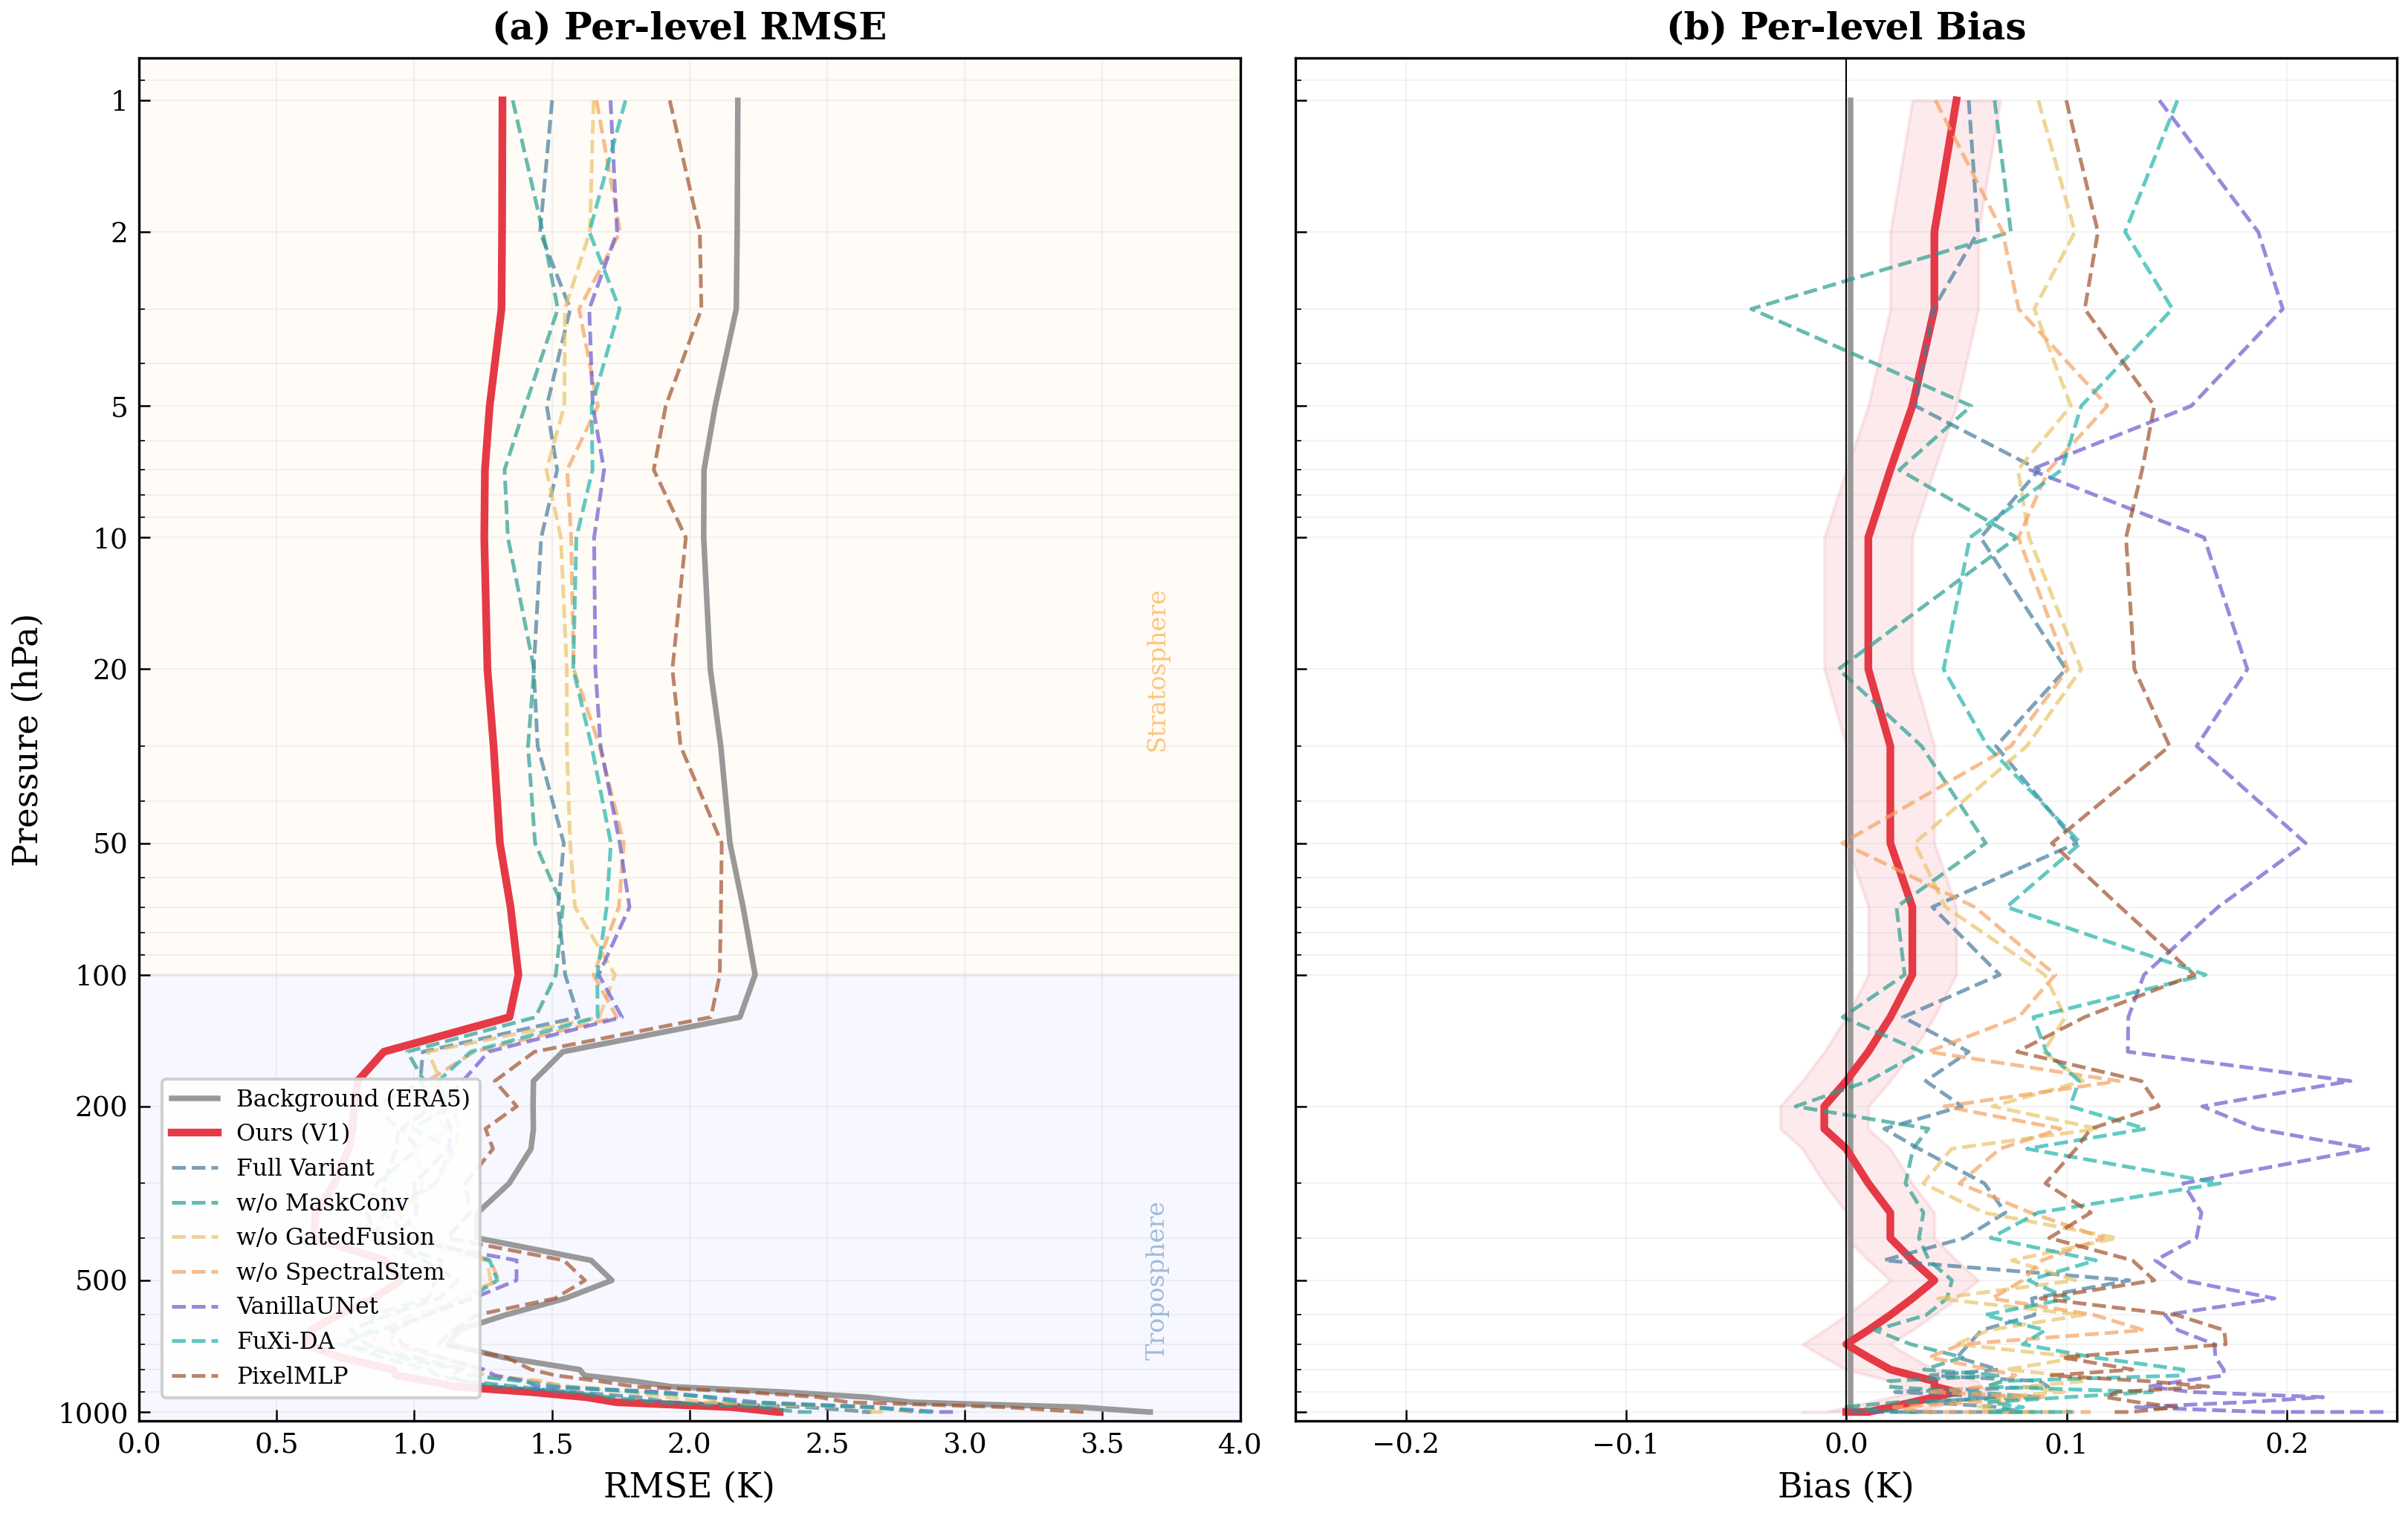
\includegraphics[width=0.70\linewidth]{../prediction/paper_figures/fig3_per_level_profile.png}
\caption{Vertical pressure-level RMSE profiles.}
\label{fig:vertical}
\end{figure}

\begin{figure}[H]
\centering
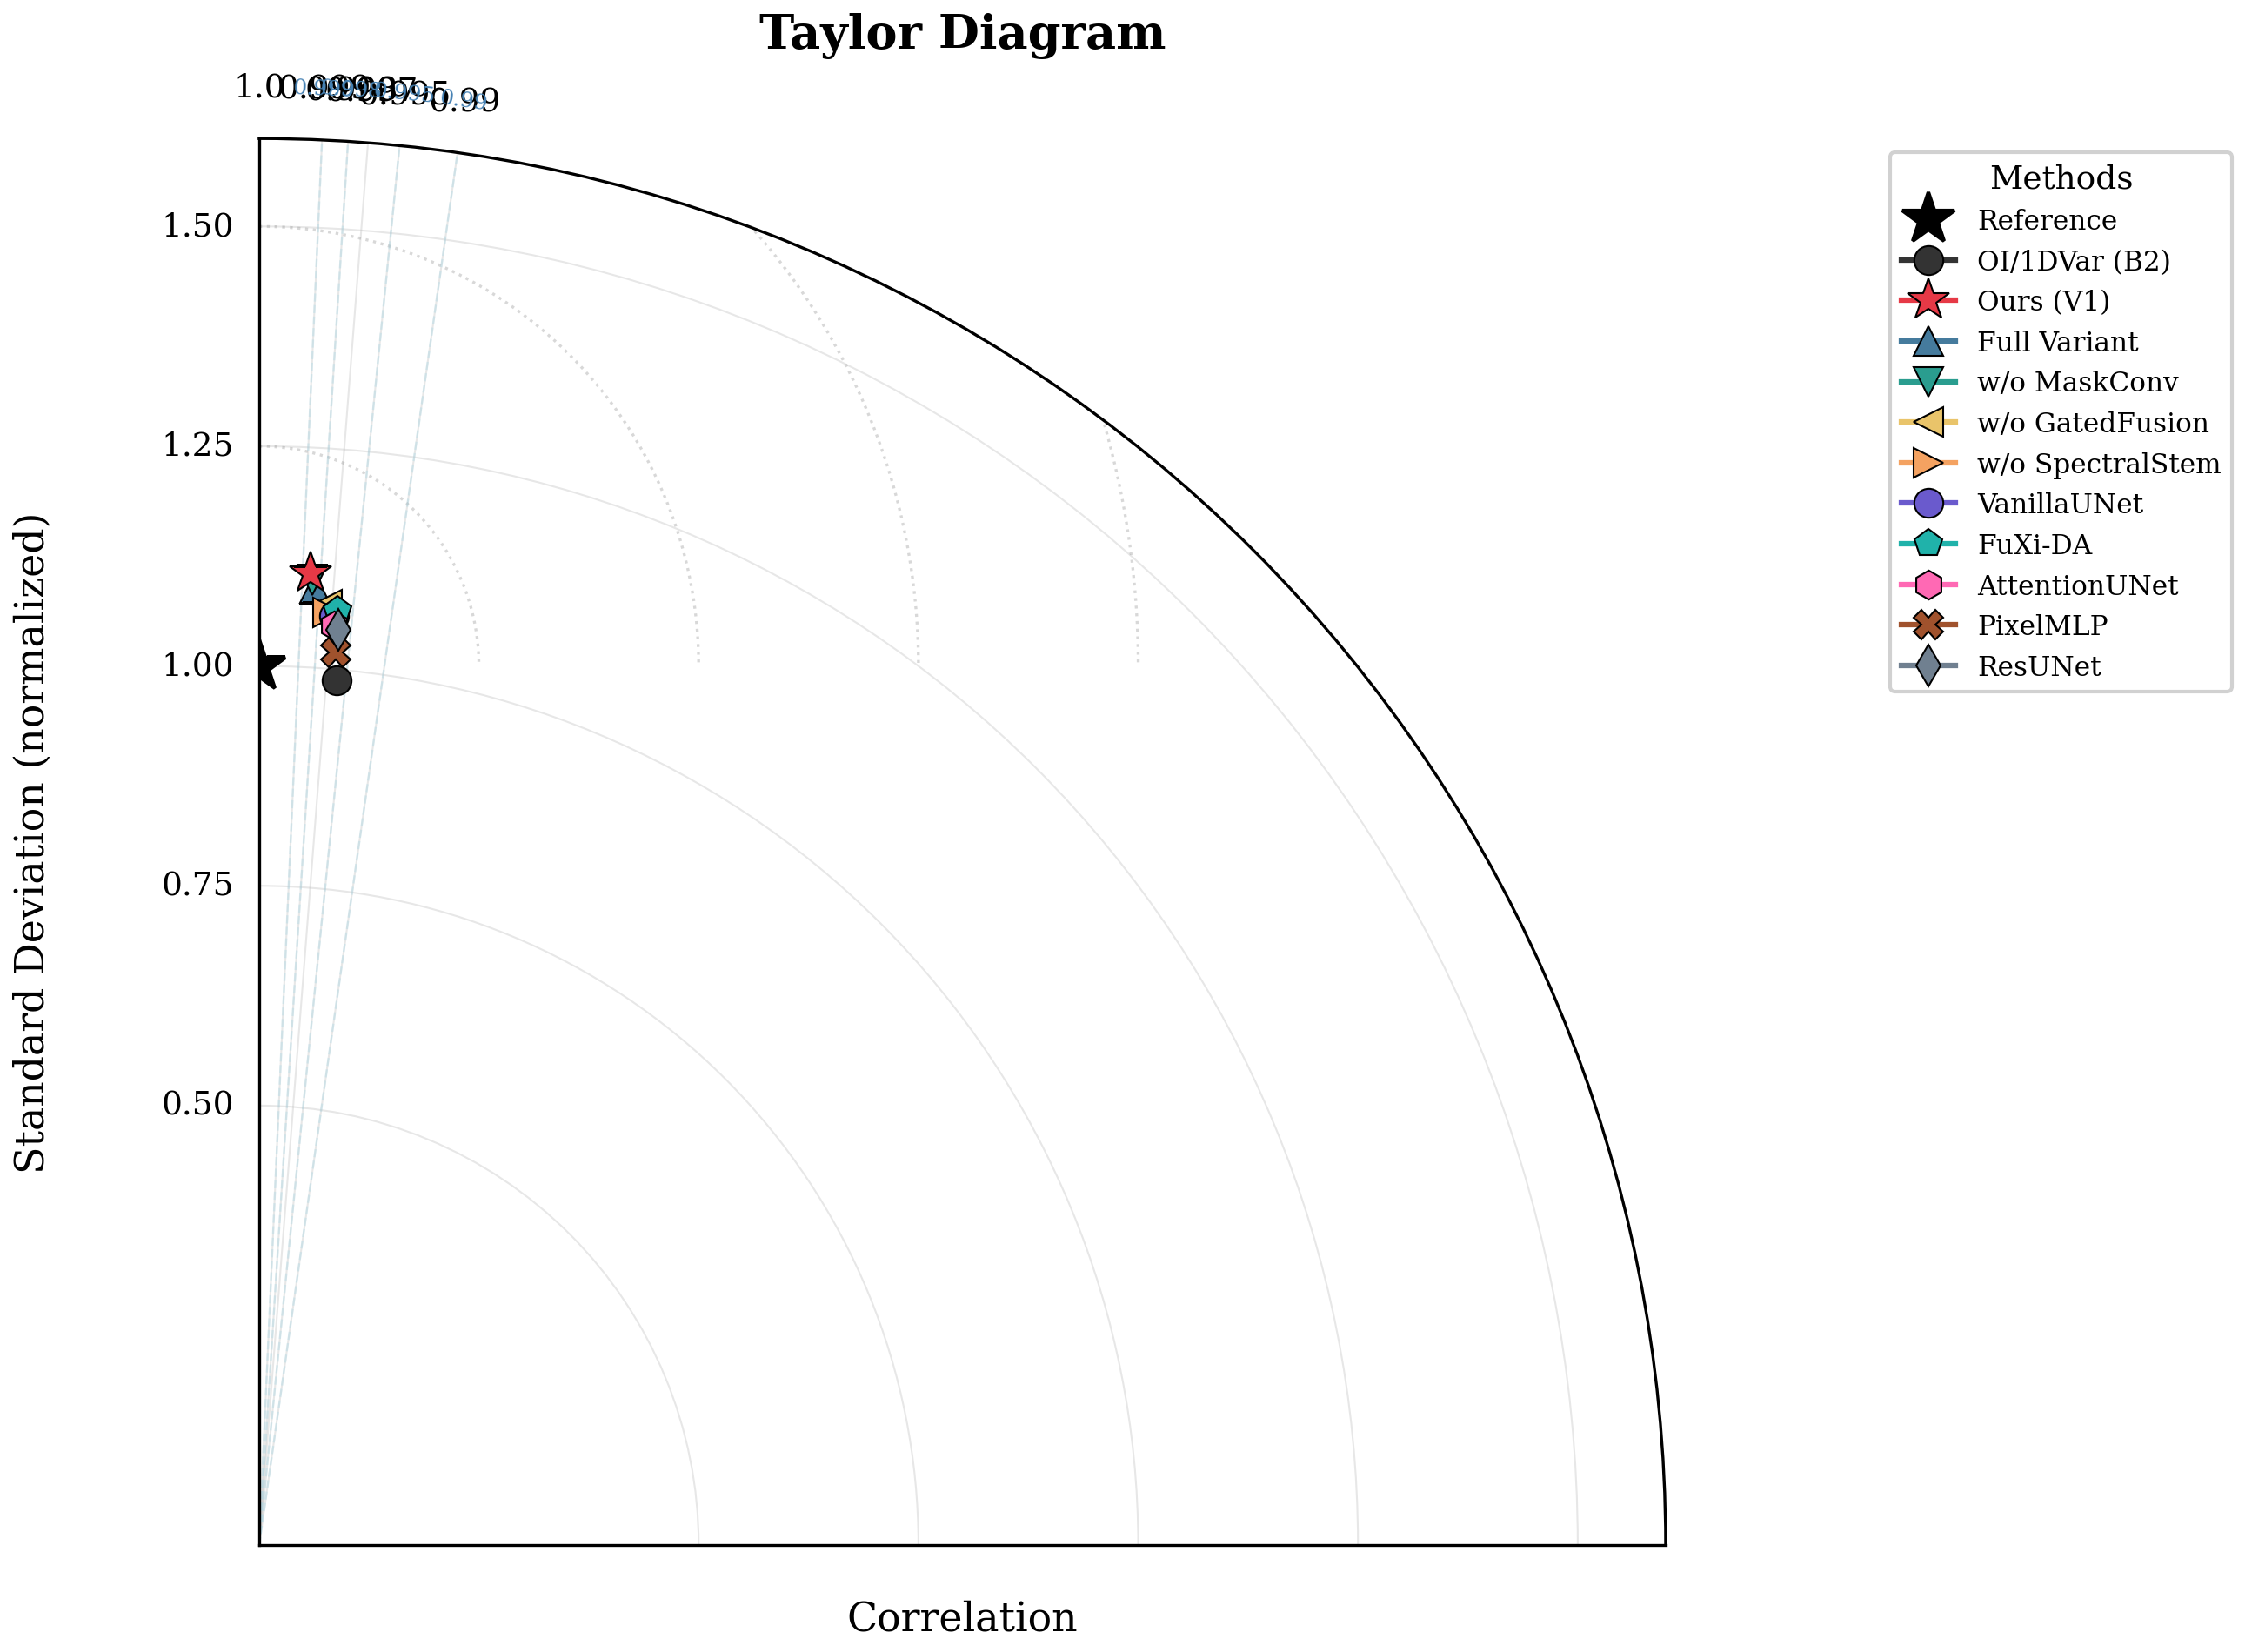
\includegraphics[width=0.72\linewidth]{../prediction/paper_figures/fig2_taylor_diagram.png}
\caption{Taylor diagram for global agreement characteristics.}
\label{fig:taylor}
\end{figure}

\section{Discussion}
\subsection{Why V1 is stronger than Full in this setup}
The code and metrics suggest the auxiliary pathway may introduce unnecessary degrees of freedom for 64x64 local patches, where large-scale geographic variation is weaker. This can slightly harm generalization compared with the leaner V1 design.

\subsection{Practical recommendation}
For this domain scale, V1 should be reported as the main model and Full should be presented as an extended variant. For larger spatial contexts (e.g., 128x128 or broader), re-testing auxiliary inputs remains important.

\subsection{Limitations}
Current draft focuses on one primary spatial setting and one test split. Future work should include multi-season robustness, uncertainty calibration, and direct impact assessment in forecasting cycles.

\section{Conclusion}
We presented a reproducible, physics-guided deep assimilation framework with comprehensive ablation and baseline comparisons. The method consistently improves over background and classical OI in the tested setup. Empirically, the best-performing variant is V1 (without auxiliary branch), which should be considered the primary architecture for this scale. The draft is directly aligned with generated figures and can be extended into a submission-ready Neurocomputing manuscript.

\section*{Reproducibility Checklist}
\begin{itemize}[leftmargin=*]
\item Codebase: distributed training script, backbone, and evaluation scripts are integrated.
\item Metrics: RMSE, MAE, Bias, Corr, level-wise RMSE.
\item Artifacts: results table and figures generated under \texttt{prediction/paper_figures}.
\item Model set: Full, V1--V4, B2--B7 all listed in evaluation mapping.
\end{itemize}

\section*{Data Availability}
The processed NPZ datasets and experiment artifacts are available in the project workspace and can be provided upon reasonable request.

\section*{Declaration of Competing Interest}
The authors declare that they have no known competing financial interests or personal relationships that could have appeared to influence the work reported in this paper.

\end{document}
